\begin{XeClass}{FTPInputStream}
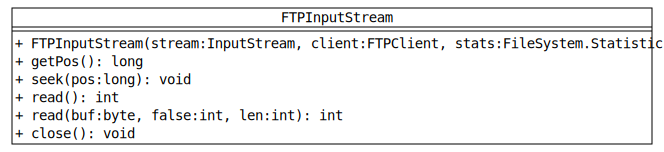
\includegraphics[width=10cm]{cdig/FTPInputStream.png}
     
 FTPInputStream继承自FsInputStream类
 并重写了InputStream接口中的各种方法

    \begin{XeMethod}{\XePublic}{FTPInputStream}{FTPInputStream}
         
 构造函数接收一个InputStream对象作为第一参数
 并且判断,当InputStream对象为null的时候则throw IllegalArgumentException("Null InputStream")
 接收FTPClient对象作为第二参数
 当FTPClient对象为null或者FTPClient对象连接没有建立的时候
 则throw IllegalArgumentException("FTP client null or not connected")

    \end{XeMethod}

    \begin{XeMethod}{\XePublic}{long}{getPos}
         

    \end{XeMethod}

    \begin{XeMethod}{\XePublic}{void}{seek}
         

    \end{XeMethod}

    \begin{XeMethod}{\XePublic \\ \XeSync}{int}{read}
         
 使用线程安全(synchronized)的read,当从wrappedStream.read()读取的字节数大于0的时候,pos值记录读入的字节数增一
 FileSystem.Statistics类用来保存与一个文件系统相关的统计信息,主要包括从该文件系统读取和写入的总的字节数
 当FileSystem.Statistics对象非空并且读入字节数不为零时,更新统计信息

    \end{XeMethod}

    \begin{XeMethod}{\XePublic \\ \XeSync}{int}{read}
         
 使用线程安全(synchronized)的read,当从wrappedStream.read()读取的字节数大于0的时候,pos值记录读入的总字节数值
 FileSystem.Statistics类用来保存与一个文件系统相关的统计信息,主要包括从该文件系统读取和写入的总的字节数
 当FileSystem.Statistics对象非空并且读入字节数不为零时,更新统计信息

    \end{XeMethod}

    \begin{XeMethod}{\XePublic \\ \XeSync}{void}{close}
         
 使用线程安全(synchronized)的close方法,调用超类的方法关闭InputStream流,closed赋值为True
 若FTPClient对象没有连接,抛出FTPException("Client not connected")
 然后关闭FTPClient连接

    \end{XeMethod}

\end{XeClass}
